\section{Results}

\subsection{Span Annotation}
For span annotation, we sought to generate useful embeddings with as little fine-tuning as possible. However, we were unable to find models that can fit BERT embeddings without some fine-tuning (see appendix [\ref{adpx:need_to_fine_tune}] for details). As a result, we decided that a small amount of fine-tuning would be necessary.

\subsubsection{BERT fine-tuning as baseline}
To establish a baseline, we fine-tuned BERT for up to 6 epochs with results shown in Figure [\ref{apdx:BERT_fine_tuning_span_annotation_sec}]. We measure performance for every 10th of a fractional epoch between 0 and 1 epochs, as well as full epochs up to 6. We observed that performance peaked at 2 epochs, achieving an Exact Match (EM) of 0.747, and an F1 score of 0.792. Between 0 and 1 epochs, performance consistently increased as measured by  both EM and F1. (For comparison with other published works, see appendix [\ref{apdx:comparison_with_devlin}]) For span detection we extracted embeddings at 3/10 of an epoch and at one full epoch. (for a rationale for this decision see appendix [\ref{apdx:explanation_of_input_embeddings_shape}])

\subsubsection{Models trained at 3/10 epoch embeddings}
Using the embeddings at 3/10 of an epoch, we explored over 20 parameter-efficient models using a combination of CNNs, pooling, and compression techniques. \footnote{See appendix [\ref{apdx:model_training_strategy}] for training time and strategy} Table [\ref{tbl:qa_3_10_Models}] shows that our best models outperform baseline BERT fine-tuned to 3/10 of an epoch. Results of all models are in appendix [\ref{apdx:span_annotation_all_results}].

First, we compare two models that use different pooling strategies, LP (learned pooling) and AP (average pooling) [\ref{sec:methods}]. We found that the LP model achieved similar performance as BERT itself, while AP significantly reduced performance. An analysis of the learned weights suggests that a non-uniform distribution of pooling weights is optimal, with the distribution slightly favoring later layers of BERT compared to earlier layers (see appendix [\ref{apdx:where_to_extract_embeddings}]).

Next, we evaluated models leveraging adapters (see Methods). We found that our modified adapters of all flavors improved model performance compared to baseline BERT at 3/10 of an epoch, with our best model improving EM by 4.5 percentage points, and F1 by 3.8. As indicated in Table [\ref{tbl:qa_3_10_Models}], without weight-sharing, the number of parameters increases by $\sim$24x, with a penalty to model performance, making weight-sharing superior in every respect. In addition, \cite{DBLP:journals/corr/abs-1902-00751} found that an adapter size of 64 provides the best F1-score when used between transformer blocks. Our modified implementation did not perform well at this size with or without weight-sharing.

While we extensively explored stacking pooling with adapters and CNNs, we did not find a model which performed better than our best adapter model. Table [\ref{tbl:qa_3_10_Models}] shows the results, and the appendix [\ref{apdx:span_annotation_all_results}] contains the rest. For one model where we stacked a modified Xception network, the number of parameters increased by 16x, but performance was no better than pooling alone.
\begin{table}[ht]
	\centering
	\small
	\begin{tabular}{L{2.9cm}|C{1.5cm} C{0.9cm} C{0.9cm}}
		\toprule
		\textbf{Model} & \textbf{\% Params} & \multicolumn{2}{c}{\textbf{SQuAD2.0}}\\
		 & \textbf{BERT}$_{large}$ & \textbf{EM} & \textbf{F1}\\
		\midrule
		BERT $\frac{3}{10}e$ & 100\% & $0.654$ & $0.702$ \\
		learned pooling (LP) & 0.001\% & $0.675$ & $0.721$ \\
		average pooling (AP) & 0.001\% & $0.657$ & $0.700$ \\
		\textbf{adapter size 386} & \textbf{0.124}\% & \boldmath$0.699$ & \boldmath$0.740$ \\
		\hspace{0.5em} - weights not shared & 2.957\% & $0.676$ & $0.723$ \\
		adapter size 64 & 0.021\% & $0.680$ & $0.732$ \\
		\hspace{0.5em} - weights not shared & 0.491\% & $0.684$ & $0.716$ \\
		LP adapter size 386 \& xception & 1.970\% & $0.668$ & $0.711$ \\
		\bottomrule
	\end{tabular}
	\caption{\label{tbl:qa_3_10_Models}Models trained on embeddings at $\frac{3}{10}$ epochs}
\end{table}

\subsubsection{Best models on top at 1 epoch}
Using 1 epoch embeddings as our training data, we fit the same set of models as with the 3/10 epoch embeddings (see the appendix [\ref{apdx:span_annotation_all_results}] for full results). In most cases, we found that our models outperformed BERT at the same level of fine-tuning. The best model is nearly identical to that found with 3/10 epoch embeddings (see table [\ref{tbl:qa_dev_set_performance}]), outperforming BERT by 2.1 percentage points in EM, and 1.3 in F1. This model’s performance is also competitive with maximum performance achieved with BERT on this task, which is BERT fine-tuned to 2 epochs. This result shows that we are able to reduce BERT fine-tuning by 1 epoch and still achieve comparable performance with a model of only about 0.124\% of the number of BERT parameters. The implications of our findings suggest that near-optimal BERT performance can be achieved in a fraction of the training time and GPU/TPU expense. 
\begin{table}[ht]
	\centering
	\small
	\begin{tabular}{L{2.9cm}|C{1.5cm} C{0.9cm} C{0.9cm}}
		\toprule
		\textbf{Model} & \textbf{\% Params} & \multicolumn{2}{c}{\textbf{SQuAD2.0}}\\
		& \textbf{BERT}$_{large}$ & \textbf{EM} & \textbf{F1}\\
		\midrule
		BERT $1e$ & 100\% & $0.728$ & $0.777$ \\
		BERT $2e$ (\textit{best}) & 100\% & $0.747$ & $0.792$ \\
		\textbf{adapter size 386} & \textbf{0.124}\% & \boldmath$0.749$ & \boldmath$0.790$ \\
		\hspace{0.5em} - weights not shared & 2.957\% & $0.716$ & $0.767$ \\
		adapter size 64 & 0.021\% & $0.739$ & $0.785$ \\
		\hspace{0.5em} - weights not shared & 0.491\% & $0.736$ & $0.784$ \\
		LP adapter size 386 \& xception & 1.970\% & $0.741$ & $0.786$ \\
		\bottomrule
	\end{tabular}
	\caption{\label{tbl:qa_dev_set_performance}Models trained on embeddings at $1$ epoch}
\end{table}

\subsubsection{Training with less data}
The previous sections show that our models perform well compared to BERT when trained on the full dataset. However, since supervised data can be difficult to obtain, we explore whether the same performance can be achieved with significantly less data. To answer this question, we trained our best models on varying amounts of data, ranging from 0\% to 100\%. As with the full dataset, all models were trained for 1 epoch. Figure [\ref{fig:1_epoch_embeddings__adapter_386_with_skip}] shows the results. In both cases, we rapidly approach strong performance early, beating BERT at $\sim$30\% of the data. Even by 10\%, we approach peak performance. This shows that we can achieve strong performance even when using less training data. 

\begin{figure}[ht]
	\centering
	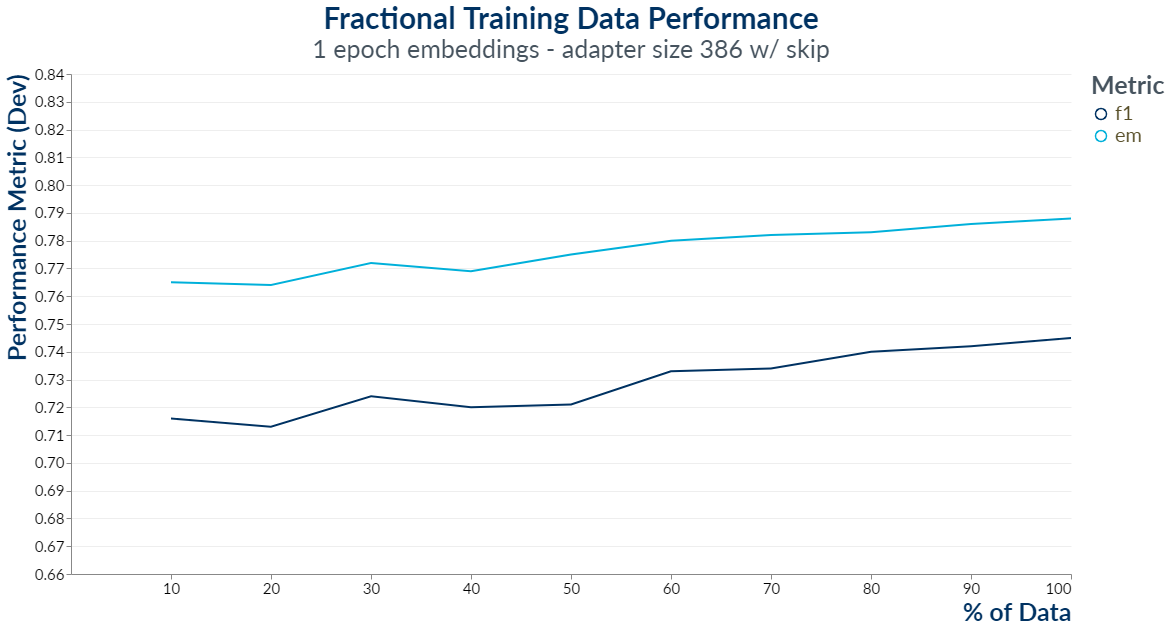
\includegraphics[width=7.5cm]{images/1_Epoch_Embeddings__Adapter_386_with_Skip.png}
	\caption{\label{fig:1_epoch_embeddings__adapter_386_with_skip}Training with less data}
\end{figure}

\subsubsection{Ensembling our models with BERT}

Since our approach requires fine-tuning BERT in order to derive workable embeddings, the BERT predictions come for free. Thus, we can ensemble our models with BERT predictions with no additional training required. Table [\ref{tbl:qa_ensembling}] presents the results of this exercise. Ensembling the models at 3/10 of an epoch did not lead to an improvement, but ensembling our 1 epoch model with BERT at 1 epoch led to more than a half percentage point improvement. This suggests that our model and BERT supply complementary information that together leads to better predictions.

\begin{table}[ht]
	\centering
	\small
	\begin{tabular}{L{4.2cm}|C{0.9cm} C{0.9cm}}
		\toprule
		\textbf{Model} & \multicolumn{2}{c}{\textbf{SQuAD2.0}}\\
		& \textbf{EM} & \textbf{F1}\\
		\midrule
		BERT $\frac{3}{10}e$     					& $0.654$  & $0.702$ \\
		our model $\frac{3}{10}e$ 					& $0.699$  & $0.740$ \\
		BERT $1e$     								& $0.728$  & $0.777$ \\
		our model $1e$ 								& $0.749$  & $0.790$ \\
		ensemble BERT+our model $\frac{3}{10}e$		& $0.691$  & $0.734$ \\
		\textbf{ensemble BERT+our model} \boldmath$1e$  & \boldmath$0.756$  & \boldmath$0.798$ \\
		\bottomrule
	\end{tabular}
	\caption{\label{tbl:qa_ensembling}QA ensembling results}
\end{table}

\subsection{Classification}

The previous section on QA span annotation uses the full sequence embeddings generated by BERT. Another common way to apply BERT is to text classification, which only uses the CLS token. Our goal in this section is to explore the efficacy of leveraging the CLS token hidden state activations in an analogous manner to our approach with the span annotation task. 

\subsubsection{BERT fine-tuning as baseline}

Similar to QA span annotation, we use BERT fine-tuning as a baseline. We fine-tuned BERT for 6 epochs using the CLS token, with the EM and F1 for each epoch shown in Figure [\ref{apdx:BERT_fine_tuning_classification}]. Our best performance was achieved at 3 epochs. We utilized embeddings at 2/10 of an epoch and 1 full epoch for the binary classification task (see appendix [\ref{adpx:need_to_fine_tune}] for rationale).

\subsubsection{Models trained at 2/10 epoch embeddings}

At 2/10ths of an epoch, BERT achieved an F1 of 0.635 and EM of 0.687 [\ref{apdx:BERT_fine_tuning_classification}]. We tried training various parameter-efficient model architectures similar to span annotation, most of which were CNN-based or simple linear. Our best performing model leverages a simple linear weighting that contracts across the channels dimension through learned weights inspired by \cite{tenney-etal-2019-bert}. We trained for 10 epochs and recorded performance of the model at each epoch evaluated against the dev set. At every epoch, the model outperformed the BERT baseline at 2/10 of an epoch [\ref{fig:bc_2_10ths_performance}].

\begin{figure}[ht]
	\centering
	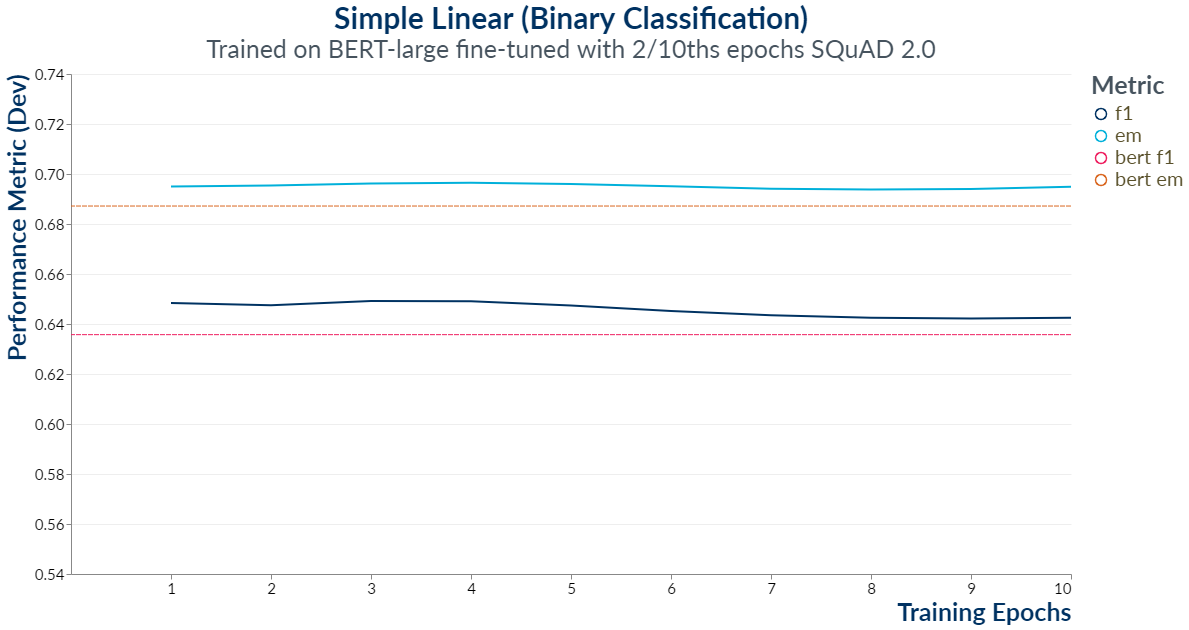
\includegraphics[width=7.5cm]{images/BinaryClassification_Tenney_Small_2_10ths_epochs_BERT_fine_tuned_Performance_plot.png}
	\caption{\label{fig:bc_2_10ths_performance}2/10ths epoch model vs BERT}
\end{figure}

\subsubsection{Models trained at 1 epoch embeddings}

With 1 epoch embeddings, our results show significant improvement over the 2/10ths epoch models. Surprisingly, the best results were achieved at 1 epoch of training with the simple linear model consisting of only 0.001\% of BERT’s parameters. This model outperforms BERT at both 1 and 2 epochs of fine-tuning. This implies that our parameter efficient model can save on 1 full epoch of BERT fine-tuning. However, performance does fall short of maximal BERT performance achieved at 3 epochs, and we were unable to find a model architecture that achieves this [\ref{tbl:bc_best_models}]. Nevertheless, this suggests that with text classification, we can use the CLS token hidden state activations in the same way we used the full sequence hidden state activations in the span annotation task. 

\begin{table}[ht]
	\centering
	\scriptsize
	\begin{tabular}{C{0.17cm}|C{0.7cm} C{0.7cm}|C{0.7cm} C{0.7cm}|C{1cm} C{1cm}}
		\toprule
		\boldmath$e$ & \textbf{BERT F1} & \textbf{BERT EM} & \textbf{Our F1} & \textbf{Our EM} & \textbf{F1 $\Delta$} & \textbf{EM $\Delta$} \\
		\midrule
		$1$ & \textcolor{berkeleyblue}{$0.720$} & \textcolor{berkeleyblue}{$0.761$} & $0.763$ & $0.782$ & \textcolor{laplane}{\boldmath$+0.043$} & \textcolor{laplane}{\boldmath$+0.021$} \\
		$3$ & \textcolor{berkeleyblue}{$0.790$} & \textcolor{berkeleyblue}{$0.804$} & $0.795$ & $0.811$ & \textcolor{laplane}{\boldmath$+0.005$} & \textcolor{laplane}{\boldmath$+0.007$} \\
		\bottomrule
	\end{tabular}
	\caption{\label{tbl:bc_best_models}Comparison of BERT and our models performance at 1 and 3 epochs on binary classification task}
\end{table} 

\subsubsection{Modeling with 3 full epoch embeddings}

BERT achieved its best performance against the SQuAD 2.0 binary classification task at 3 full epochs (0.79 F1, 0.804 EM) [\ref{apdx:BERT_fine_tuning_classification}].  Given that the simpler linear model outperformed BERT at the same level of fine-tuning, we wanted to evaluate if the simple model’s trend in performance would continue as BERT exhausts its ability to learn the binary classification task.  In this final evaluation, the linear model again outperformed BERT, achieving the top overall score for our task, albeit at a smaller margin [\ref{tbl:bc_best_models}].